\section{Simulation Model Description}

In this section the Arena model is described and explained. 
The model has been split into two models, firstly the management of the cashiers (main model) and secondly the management of the vehicles (submodel Pumps). 
The main model can be found in \autoref{fig:main}. 
Larger images can be found in \autoref{app:modeldescription}. 
The main model and sub model are described briefly in this section.
The detailed explanations can be also be found in \autoref{app:modeldescription}.  
\begin{figure}[h!]
\begin{center}
	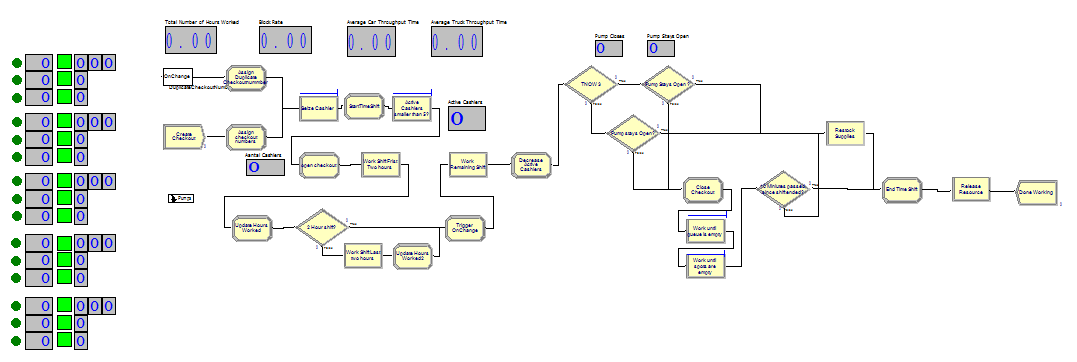
\includegraphics[scale=0.6]{images/model-description/main}
	\caption{Arena Main Model}
	\label{fig:main}
\end{center}
\end{figure}
\subsection{Main Model Cashier management}
The main model is the model which describes the cashier management. 
It creates five checkouts at the start, these checkouts are the entities that go through the system. 
When cashiers arrive they are put in a set of available cashiers and the checkouts seize a cashier. 
When a cashier is seized the checkout opens its associated lanes for 4 hours and after that it is decided if another cashier takes over or if the checkout closes. 
If it closes all the vehicles currently in the lane will be served and then the cashier leaves. 
If another cashier takes over the checkout the old cashier restocks the supplies and then leaves. 
Just before the cashier finishes her shift, a duplicate of the checkout is created, since the old entity of this checkout leaves the system after the shift. 
The duplicate behaves the same as the old entity and the model continues with still five checkouts. 

\subsection{Vehicle management}
The other (sub)model in is the vehicle management model. 
This model models the arrival of vehicles at the fuel station and how these vehicles pass through the model. 
A detailed figure of the model can be found in \autoref{fig:modelpumps} in \autoref{app:modeldescription}. 
In this submodel, an entity is created for every vehicle.
This entity first checks if one of the open lanes has enough space so the vehicle can enter it. 
If multiple of these lanes have enough space the entity chooses the shortest lane. 
After that it waits for its turn, refuels and joins the queue for the cashier. 
This queue is special, because in that queue three lanes merge into one. When the vehicle paid the cashier it leaves the model and the queue is updated. 

\subsection{Resource schedules, variables and attributes}
All the resource schedules, variables and attributes which have been used in these models are described in \autoref{app:modeldescription}.